\chapter{Perspectives et améliorations possibles d'IBIS : une synthèse après un an de développement}\label{ch:resultats-et-failles-d'ibis-:-une-synthese-apres-un-an-de-developpement2}\label{ch:resultats-et-failles-d'ibis-:-une-synthese-apres-un-an-de-developpement}
%- L'uniformisation est perfectible (bouts de code dupliqués, notamment à cause de la généralisation des modèles $RC$)
%- ID par défaut du modèle $RC$ dans un calcul = 1, prête à confusion
%
%## État des lieux
%
%- Résolution d'équations différentielles
%- Euler explicite = pas de garantie de convergence et explosion sur certains cas
%- Remplacé par solveur Radau/BDF/RK45 = beaucoup plus lent, problématique dans le cas d'une optimisation
%- Compromis à trouver, peut-être réimplenter Euler avec vérification de la convergence et passage sur Radau si ce n'est pas le cas ?
%- => essayer diffrax qui utilise le framework Jax
% Pb des conditions initiales pour la résolution
%- Méthodes auto-régressives très prometteuses tant sur la précision que la performance mais peu explorées
%- Méthode 3CL éminement liée aux paramètres $RC$ et pourtant pas implémentée
%- Architecture données discutable (SQLite est le choix de la facilité, DuckDB semble plus adapté notamment pour une séparation propre des entrées et sorties)
%- CI
%- Analyse de données
%
%### Amélioration de l'aspect CI/CD

\section{}\label{sec:etat-des-lieux}

    \subsection{Fonctionnalités développées et considérées matures}\label{subsec:fonctionnalites-developpeeset-considerees-matures}

    \subsection{Axes d'amélioration et suite du développement}\label{subsec:axes-d'amelioration-et-suite-du-developpement}
        % TODO : Tableau tiré de snakeviz et des fichiers .prof
        %TODO: snakeviz montre un goulot d'étranglement très clair au niveau de la résolution des ODE. Des solutions doivent être trouvées pour pallier ce problème, seul problème majeur d'IBIS.
        %TODO : optimiseur des hyperparamètres blackbox (degré, lags) car les modèles ARX sont très rapides (pas d'optimisation interne des paramètres comme pour la PSO) mais sensibles à leurs hyperparamètres, lesquels ne peuvent pas être fixés car grandement dépendants d'une situation à l'autre.
        %TODO : Réseaux de Neurones et en particulier deux architectures : récurrents (citer Nature, expliquer pourquoi les réseaux de neurones peuvent être une piste) et GNN (grâce à la structure en graphe)
        %TODO : conditions initiales pour la résolution des équations (figure associée)

        \ldots La figure \ref{fig:predictionibisibbtairinit} est éloquente à cet égard.
        \begin{figure}[H] \centering
                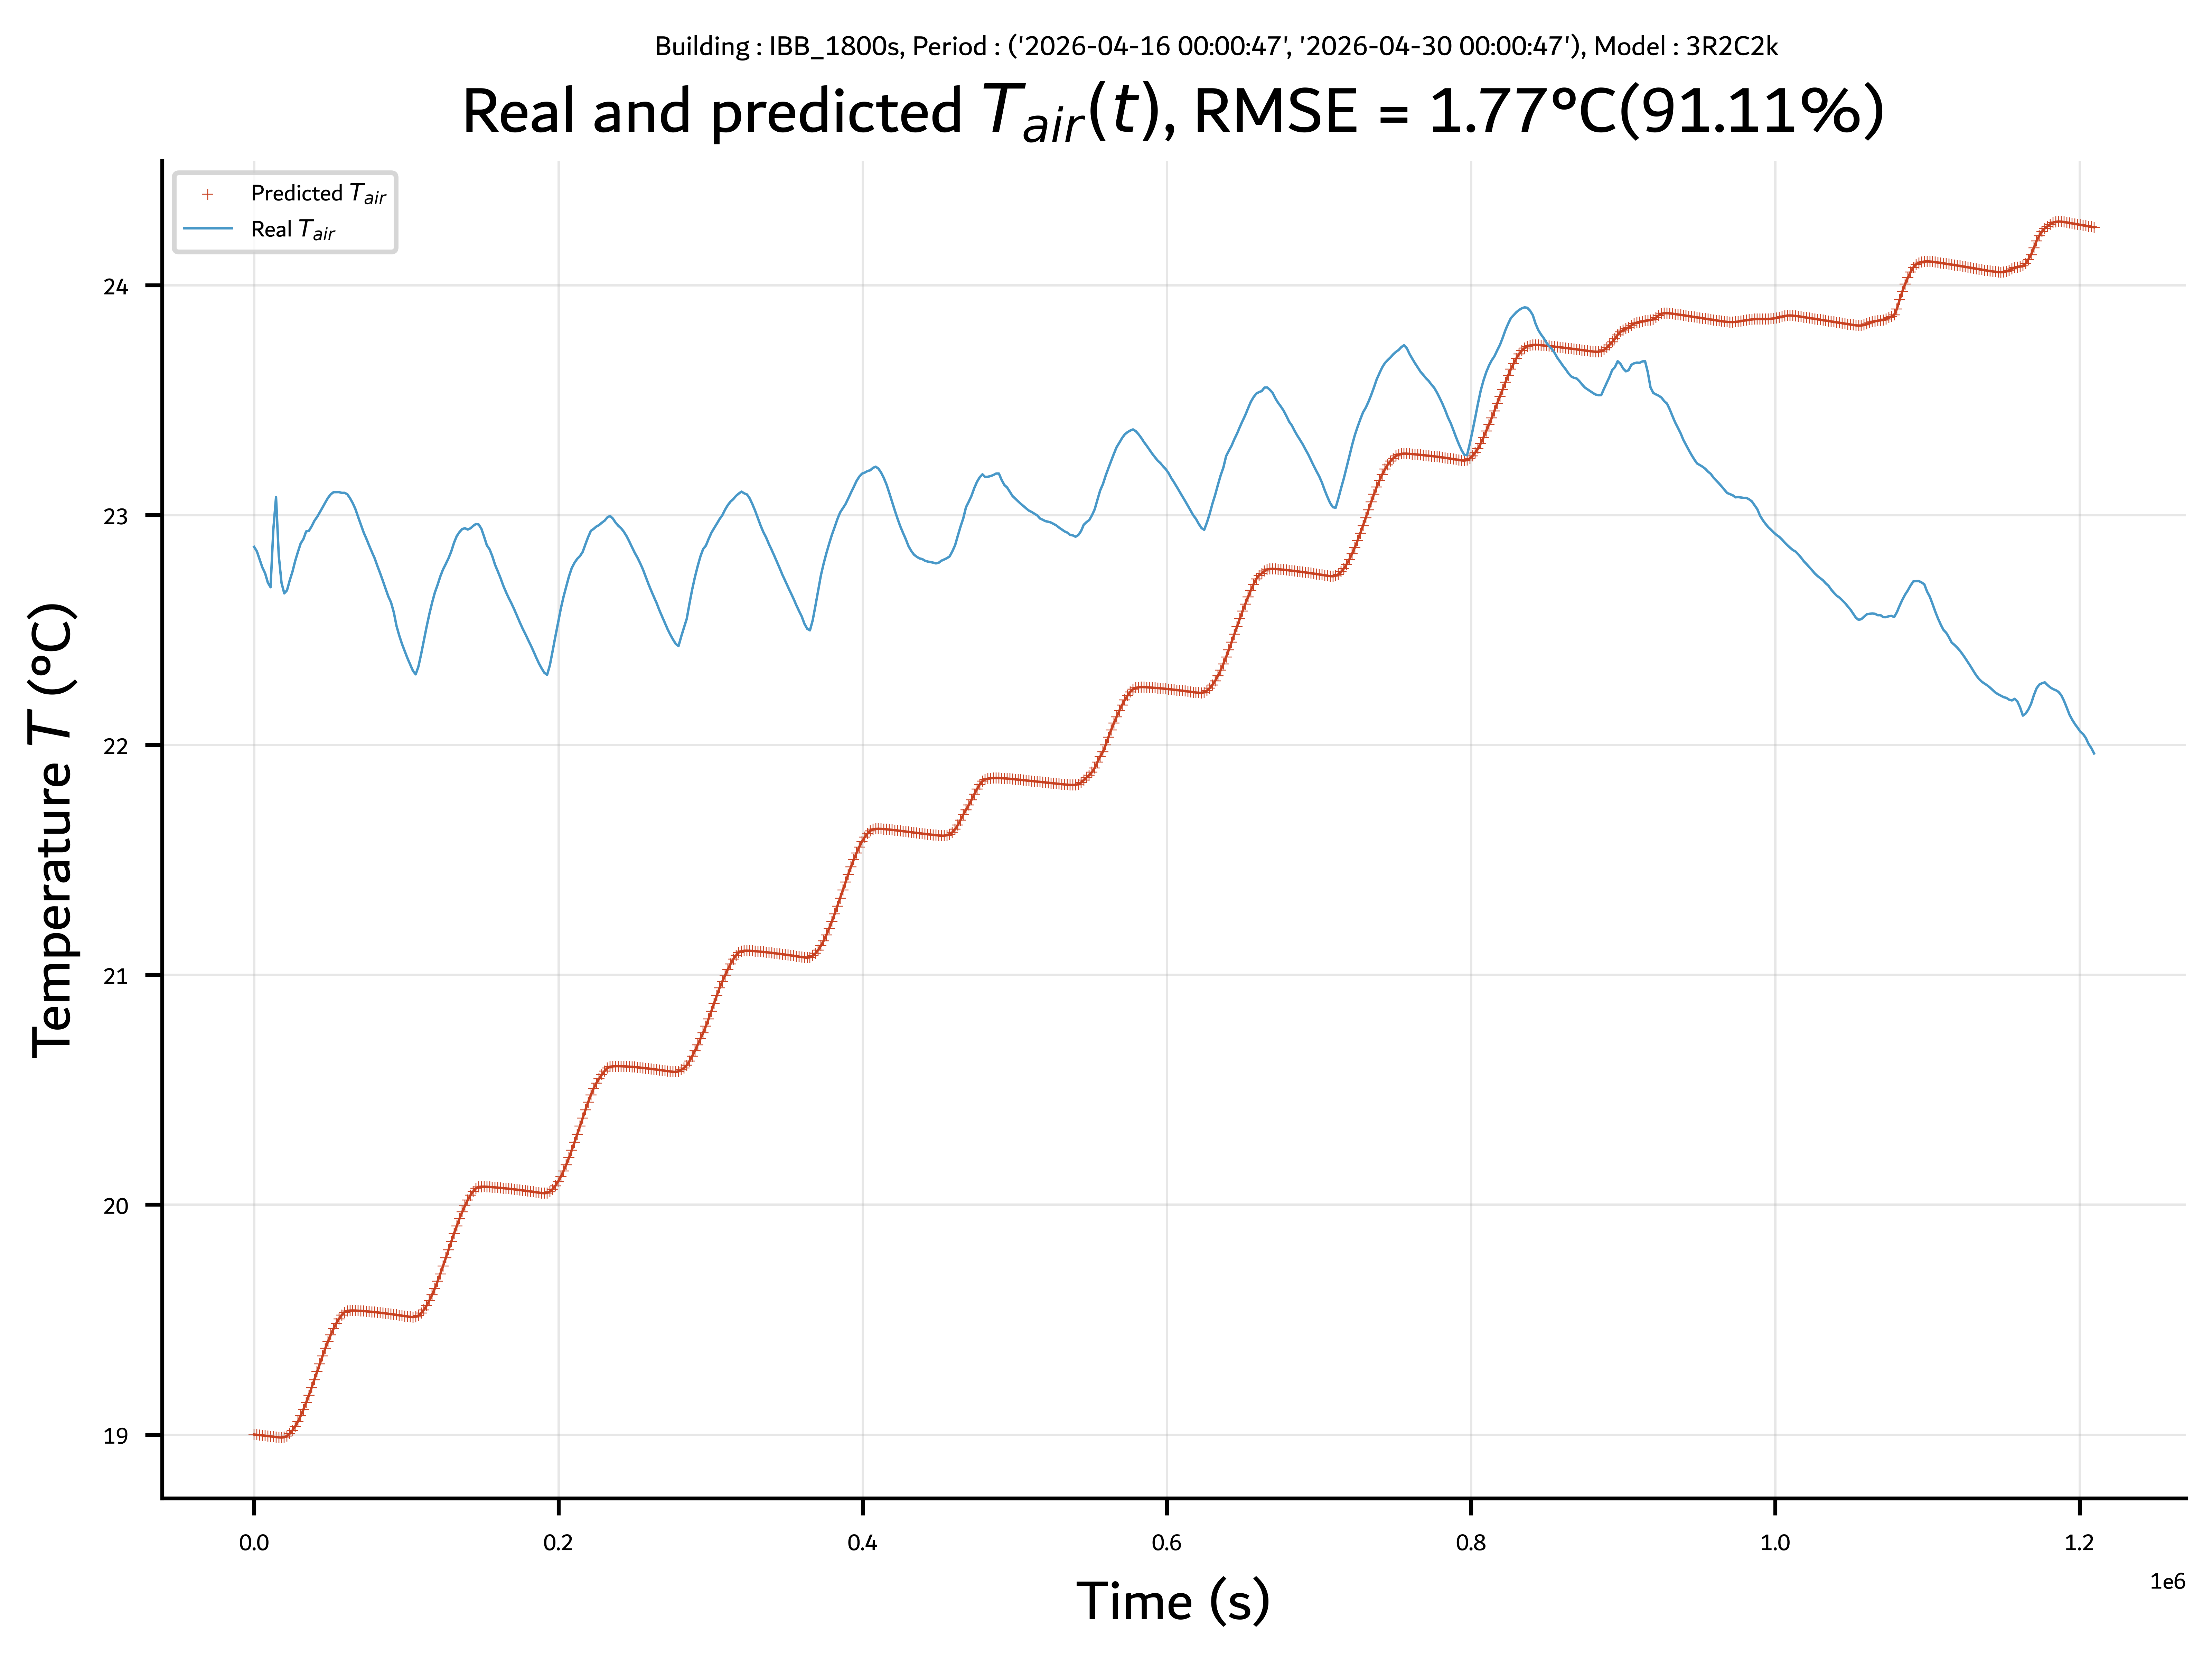
\includegraphics[width = 0.80\textwidth]{figures/diagrammes/courbes/distrisim/1121587_T_Air}
            \caption{Exemple de comparaison entre la température mesurée à l'intérieur d'IBB et les prévisions d'IBIS}\label{fig:predictionibisibbtairinit}
        \end{figure}

\section{Vers une intégration dans un groupe de projets cohérent : BEST}\label{sec:vers-une-integration-dans-un-groupe-de-projets-coherent-:-best}
% TODO : BEST